\subsection{Examples}



\begin{example2}{Selection Structures}
If-Then-Else with unsigned 8-bit variables:

\textbf{Structogram:}\\
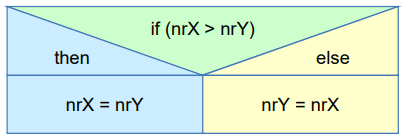
\includegraphics[width=0.7\linewidth]{images/structogramex1.png}
\vspace{2mm}\\
\begin{minipage}{0.6\linewidth}
\textbf{Flowchart:}\\
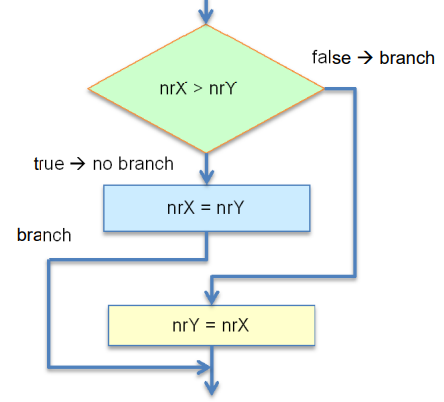
\includegraphics[width=\linewidth]{images/flowchartex1.png}
\end{minipage}
\begin{minipage}{0.38\linewidth}
\textbf{C code:}
\vspace{2mm}\\
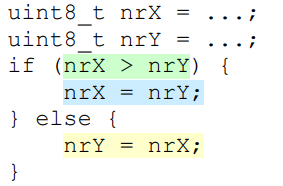
\includegraphics[width=\linewidth]{images/ccodeex1.png}
\end{minipage}

\textbf{Assembly code:}\\
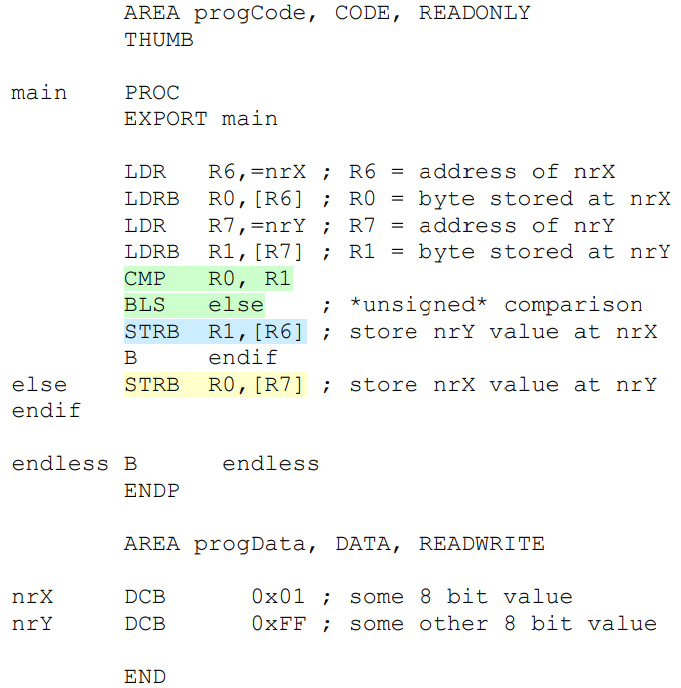
\includegraphics[width=\linewidth]{images/assemblycodeex1.png}
\end{example2}

\begin{example2}{Selection Structures}
If-Then-Else with signed 8-bit variables:
\vspace{2mm}\\
\begin{minipage}[t]{0.5\linewidth}
\textbf{Structogram:}\\
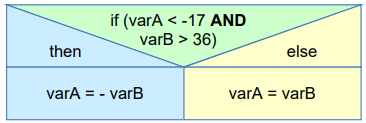
\includegraphics[width=\linewidth]{images/structogramex2.png}
\end{minipage}
\begin{minipage}[t]{0.48\linewidth}
\textbf{C code:}
\vspace{2mm}\\
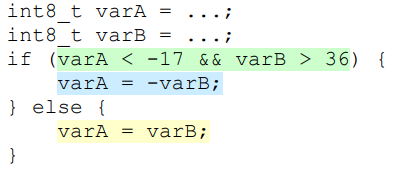
\includegraphics[width=\linewidth]{images/ccodeex2.png}
\end{minipage}

\textbf{Flowchart:}\\
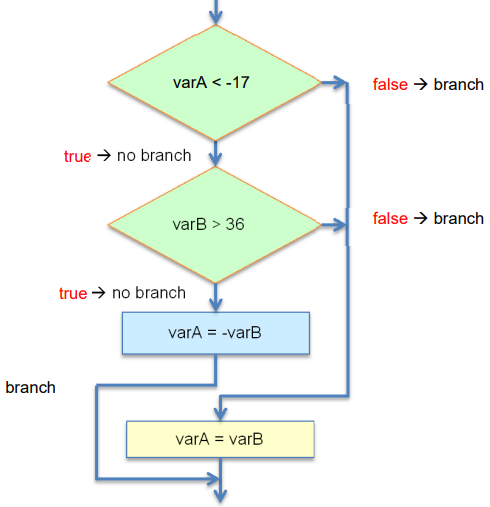
\includegraphics[width=0.7\linewidth]{images/flowchartex2.png}

\textbf{Assembly code:}\\
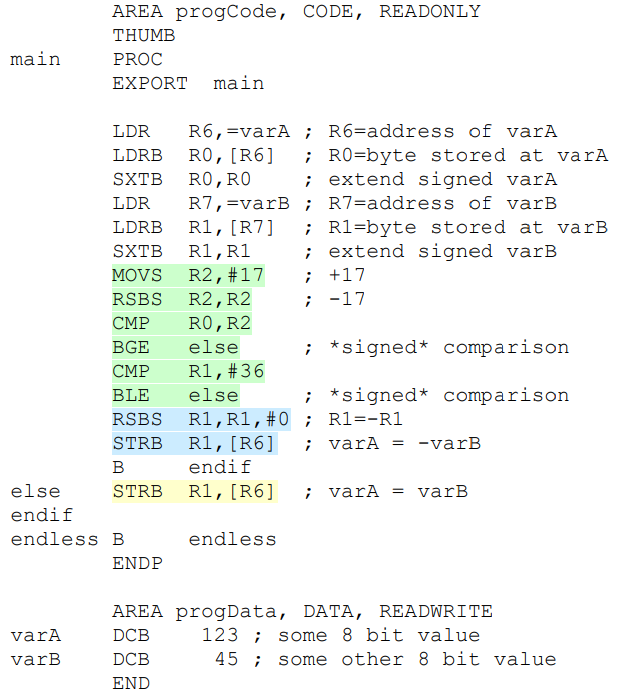
\includegraphics[width=0.9\linewidth]{images/assemblycodeex2.png}
\end{example2}

\begin{example2}{Selection Structures}
If-Then-Else with signed 16-bit variables:
\vspace{2mm}\\
\begin{minipage}[t]{0.5\linewidth}
\textbf{Structogram:}\\
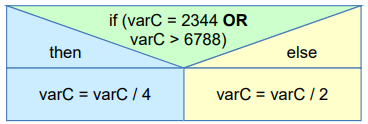
\includegraphics[width=\linewidth]{images/structogramex3.png}
\end{minipage}
\begin{minipage}[t]{0.48\linewidth}
\textbf{C code:}
\vspace{2mm}\\
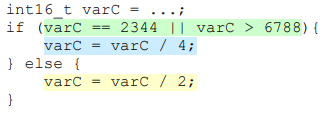
\includegraphics[width=\linewidth]{images/ccodeex3.png}
\end{minipage}

\textbf{Flowchart:}\\
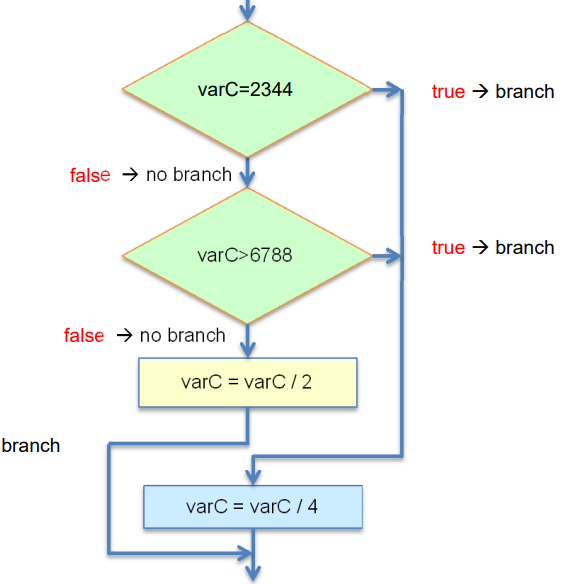
\includegraphics[width=0.7\linewidth]{images/flowchartex3.png}

\textbf{Assembly code:}\\
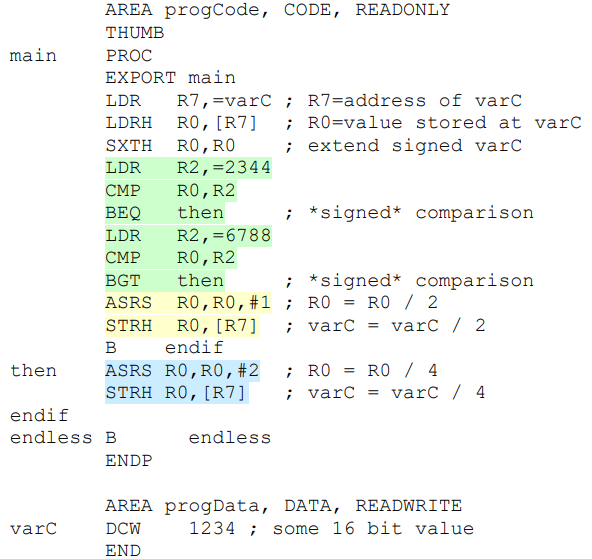
\includegraphics[width=\linewidth]{images/assemblycodeex3.png}
\end{example2}



\begin{example2}{For-Loop Implementation}\\
Example for-loop in C and assembly:

\begin{lstlisting}[language=C, style=basesmol]
// C code with volatile variables
volatile int32_t i = 0;
volatile int32_t count = 0;
for(i = 0; i < 10; i++) {
    count++;
}
\end{lstlisting}

Assembly implementation:
\begin{lstlisting}[language=armasm, style=basesmol]
    AREA    progCode, CODE, READONLY
    THUMB
main
    PROC
    EXPORT  main
    
    LDR     R6, =i          ; R6 = address of i
    LDR     R0, [R6]        ; R0 = value at i
    LDR     R7, =count      ; R7 = address of count
    LDR     R1, [R7]        ; R1 = value at count
    B       cond
    
loop
    ADDS    R0, R0, #1      ; Increment i
    ADDS    R1, R1, #1      ; Increment count
cond
    CMP     R0, #10
    BLT     loop            ; Branch if i < 10
    
    STR     R0, [R6]        ; Store final i
    STR     R1, [R7]        ; Store final count
    ENDP
\end{lstlisting}

Compiler-optimized version:
\begin{lstlisting}[language=armasm, style=basesmol]
    LDR     r1, [pc, #20]   ; Load address
    MOVS    r0, #0          ; Initialize counter
    STR     r0, [r1, #0]    ; Store i
    LDR     r2, [r1, #4]    ; Load count
    
increment
    ADDS    r0, r0, #1      ; i++
    ADDS    r2, r2, #1      ; count++
    CMP     r0, #10         ; Check condition
    BLT     increment       ; Loop if i < 10
    STM     r1!, {r0, r2}   ; Store final values
\end{lstlisting}
\end{example2}

